\section{方法}

本节详细描述了我们提出的基于一对多对应关系和对称感知的6D物体姿态估计训练方法。

我们旨在解决超越一对一对应方法的对称模糊问题。借鉴二进制编码在一对一对应方法中的成功应用\cite{2024hipose, su2022zebrapose},我们将这种方法扩展到编码一对多对应关系,然后将其输入到网络中以获得最终姿态,无需RANSAC或精细化处理。

\subsection{问题定义}

给定具有已知内参的RGB图像和一组物体的CAD模型,我们的目标是估计图像中每个物体相对于相机的姿态(旋转矩阵 $\mathbf{R} \in SO(3)$ 和平移向量 $\mathbf{t} \in \mathbb{R}^3$)。

对于非对称物体,只有一个真实姿态 $\mathbf{T}=[\mathbf{R}|\mathbf{t}]$,而对于对称物体,则有多个可能的真实姿态 $\mathbf{T}_k, k=1, 2,...,n$,其中 $n$ 是真实姿态的数量,可以是无限的。

ZebraPose\cite{su2022zebrapose} 构建了一个包含 $N$ 个物体模型顶点的二进制编码,定义了唯一对应于顶点 $\mathbf{P}_j$ 的 $d$ 位二进制代码 $\mathbf{c}_{j}$。二进制编码是通过迭代构建的,在每一步中将网格分成相等数量的顶点,并为每组分配一个位。在表面划分的第 $it$ 次迭代中,$it \in \{0, 1, \text{\textellipsis}, d-1\}$,我们有 $2^{it+1}$ 个独立的子组。给定一组顶点,划分是通过平衡的 k-means 进行的,结果形成两个子组。对于非对称物体,一对多对应关系等同于一对一对应关系,因为没有由于对称性引起的歧义。

在接下来的部分中,我们详细比较了一对一对应关系和一对多对应关系。随后,我们介绍了估计6DoF物体姿态的方法,包括从表面编码到最终姿态估计的整个过程。

\subsection{2D-3D 对应关系}
\textbf{一对一对应关系 } 提取一对一对应关系是姿态估计中的关键组成部分,它表示从观测图像中的2D点 $\mathbf{p}_i=(u_i,v_i)$ 和物体模型中的3D点 $\mathbf{P}_j=(x_j,y_j,z_j)$ 之间的匹配,记为 $\mathbf{o}_r = (\mathbf{p}_i, \mathbf{P}_j)$,其中 $\mathbf{p}_i\in \mathbb{R}^2$ 和 $\mathbf{P}_j\in \mathbb{R}^3$。对应关系可以基于逐点的真实姿态 $\mathbf{T}$ 得出:

\begin{equation}
        \mathbf{p}_i=\pi(\mathbf{T}\cdot \mathbf{P}_j) 
        \label{eq:projection}
\end{equation}

其中 $\pi(\cdot)$ 是使用内参矩阵的针孔相机模型的投影函数。我们定义了一对一对应关系集 $\mathbf{O} = \{\mathbf{o}_1, \mathbf{o}_2, ..., \mathbf{o}_m\}$,包含 $m$ 个一对一对应关系,其中 $\mathbf{o}_r = (\mathbf{p}_i, \mathbf{P}_j)$。透视-n-点(PnP)模块旨在给定一组一对一对应关系的情况下恢复姿态 $\mathbf{T}$。大多数基于对应关系的方法使用一对一对应关系集作为中间几何表示。对于非对称物体,一对一对应关系是唯一的,可以无歧义地恢复,但对于对称物体则不然。

\begin{figure}[ht]
  \centerline{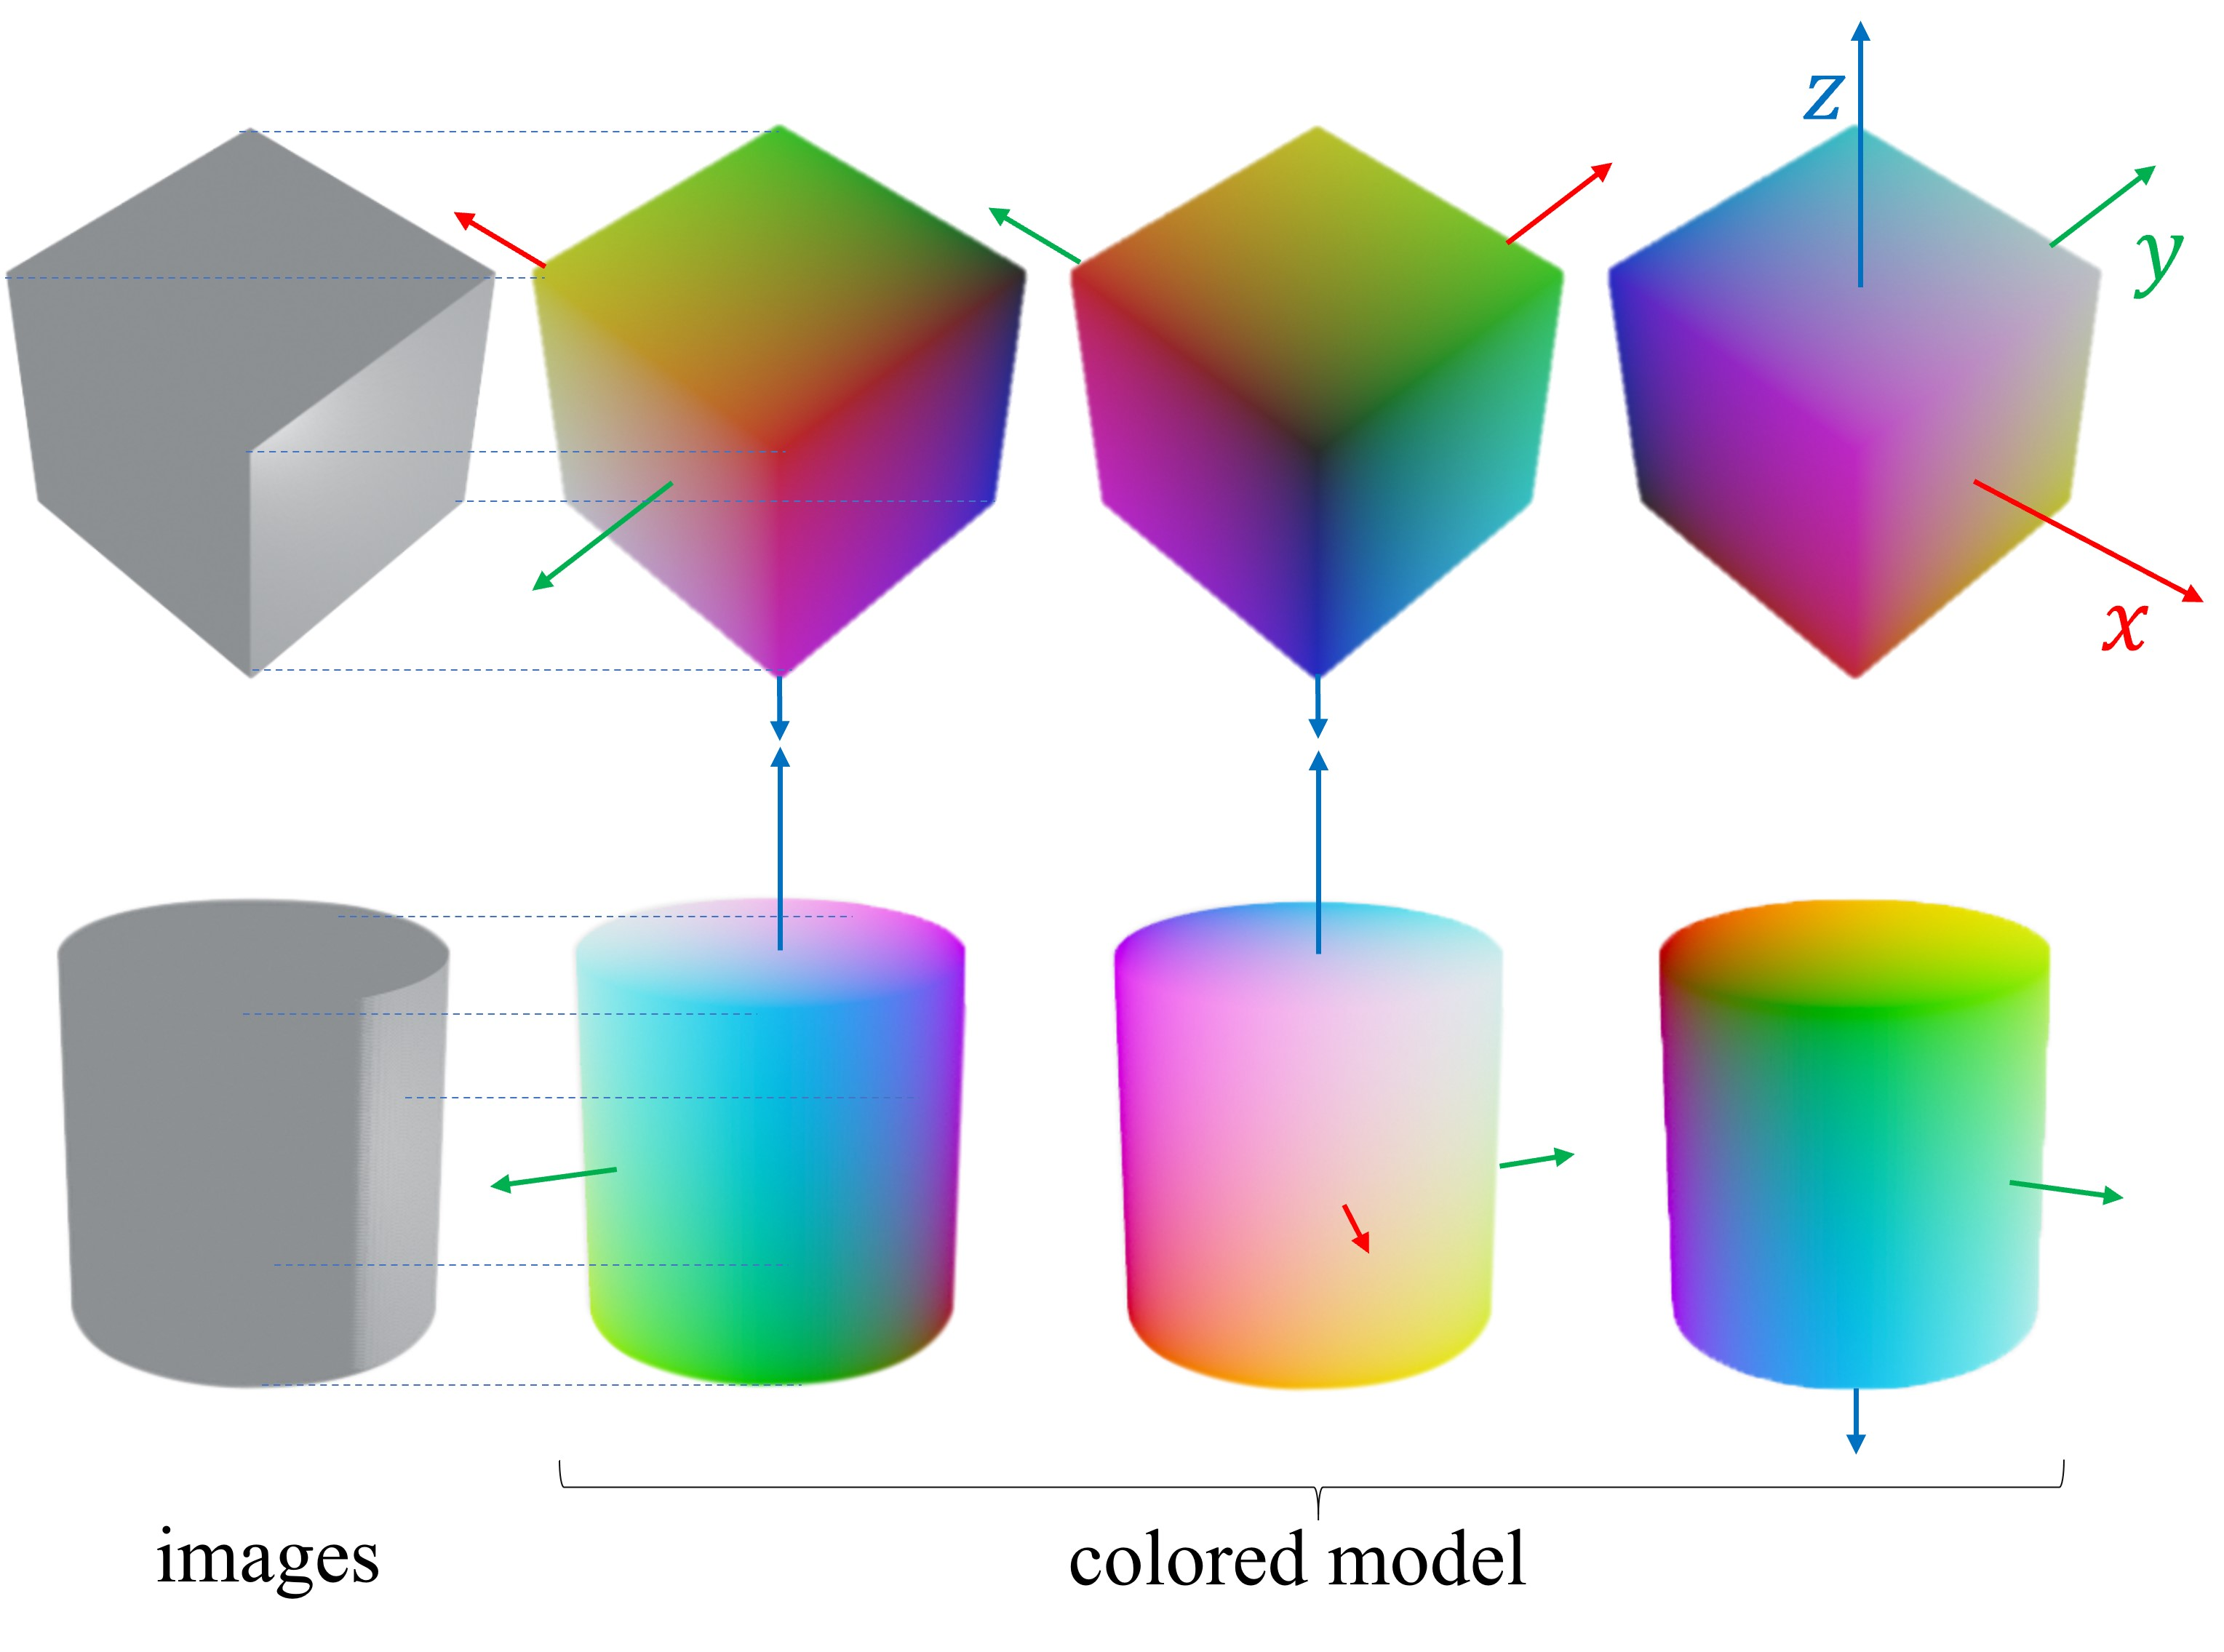
\includegraphics[width=0.75\textwidth]{figure/symnet/one-to_one-correspondence.jpg}}
  \caption{Multiple possible one-to-one correspondence sets.}
  \label{fig:one_one_corres}
\end{figure}

对于对称物体的每个真实姿态 $\mathbf{T}_k$,我们可以使用 \Cref{eq:projection} 获得一对一对应关系集。然而,在训练阶段,将具有显著不同对应关系集的相似图像设置为学习目标可能会导致收敛问题。我们在 \autoref{fig:one_one_corres} 中展示了立方体和圆柱体的不同一对一对应关系集。左列:未纹理化的立方体和圆柱体图像。顶部:立方体图像的三种可能的对应关系集。底部:圆柱体图像的三种可能的对应关系集。右三列中模型的颜色表示物体框架中的坐标,红色、绿色和蓝色分别表示 x 轴、y 轴和 z 轴的坐标。物体框架由彩色箭头表示为坐标。虚线显示了2D-3D对应关系。最佳观看模式为彩色模式。

\textbf{一对多对应关系 } 我们定义一对多对应关系来表示2D点 $\mathbf{p}_i=(u_i,v_i)$ 和所有可能的3D点集合 $\mathbf{Y}_j = \{\mathbf{P}_{j,1}, \mathbf{P}_{j,2}, ..., \mathbf{P}_{j,n}\}$ 之间的匹配,记为 $\mathbf{o}_r = (\mathbf{p}_i, \mathbf{Y}_j)$。对应关系应满足以下条件:

\begin{equation}
\mathbf{p}_i = \pi(\mathbf{T}_k \cdot \mathbf{P}_{j,k}), \quad k = 1,2,...,n
\label{eq:projection_one_to_many}
\end{equation}

$\mathbf{T}_k$ 是所有可能的真实姿态。
我们定义了一对多对应关系集 $\mathbf{O}_\text{sym} = \{\mathbf{o}_1, \mathbf{o}_2, ..., \mathbf{o}_m\}$,包含 $m$ 个一对多对应关系,其中 $\mathbf{o}_r = (\mathbf{p}_i, \mathbf{Y}_j)$,如~\Cref{fig:many_many_corres} 所示。
一对多对应关系表明,从一个像素 $\mathbf{p}_i$ 出发,不可能确定匹配的3D点坐标 $\mathbf{P}_j$,但可以确定对应的3D点集 $\mathbf{Y}_j$。与一对一对应关系相比,一对多对应关系由于其无歧义性,为网络提供了一个更容易学习的任务。

\begin{figure}[ht]
\centerline{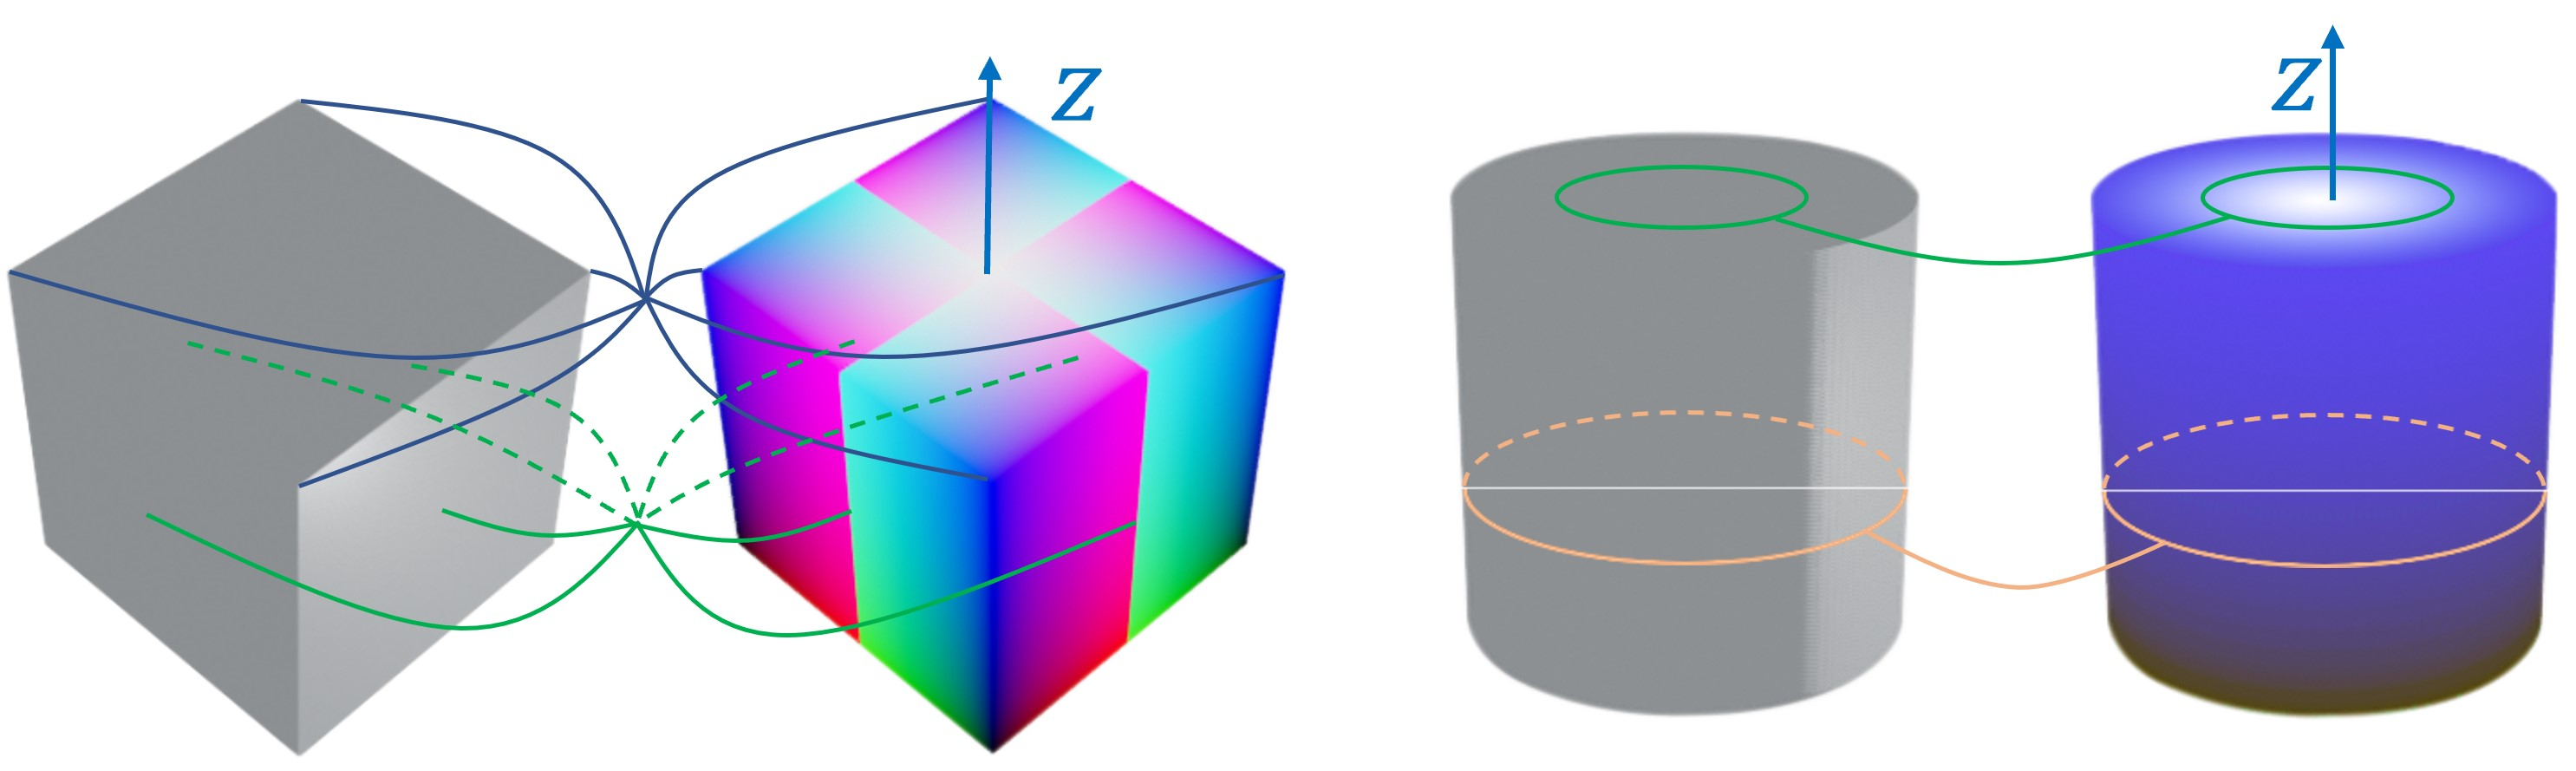
\includegraphics[width=0.75\textwidth]{figure/symnet/one-to-many-correspondence.jpg}}
\caption{\textbf{一对多对应关系集。} 一对多对应关系中的所有3D点都具有相同的颜色纹理。左图:假设立方体只有沿z轴旋转0度、90度、180度和270度的4种对称性,展示了角和侧面中心的两个特定一对多对应关系。不可见部分用虚线连接,可见部分用实线连接。右图:展示了侧面和顶部表面的两个特定一对多对应关系。}
\label{fig:many_many_corres}
\end{figure}

\begin{figure}[ht]
    \centerline{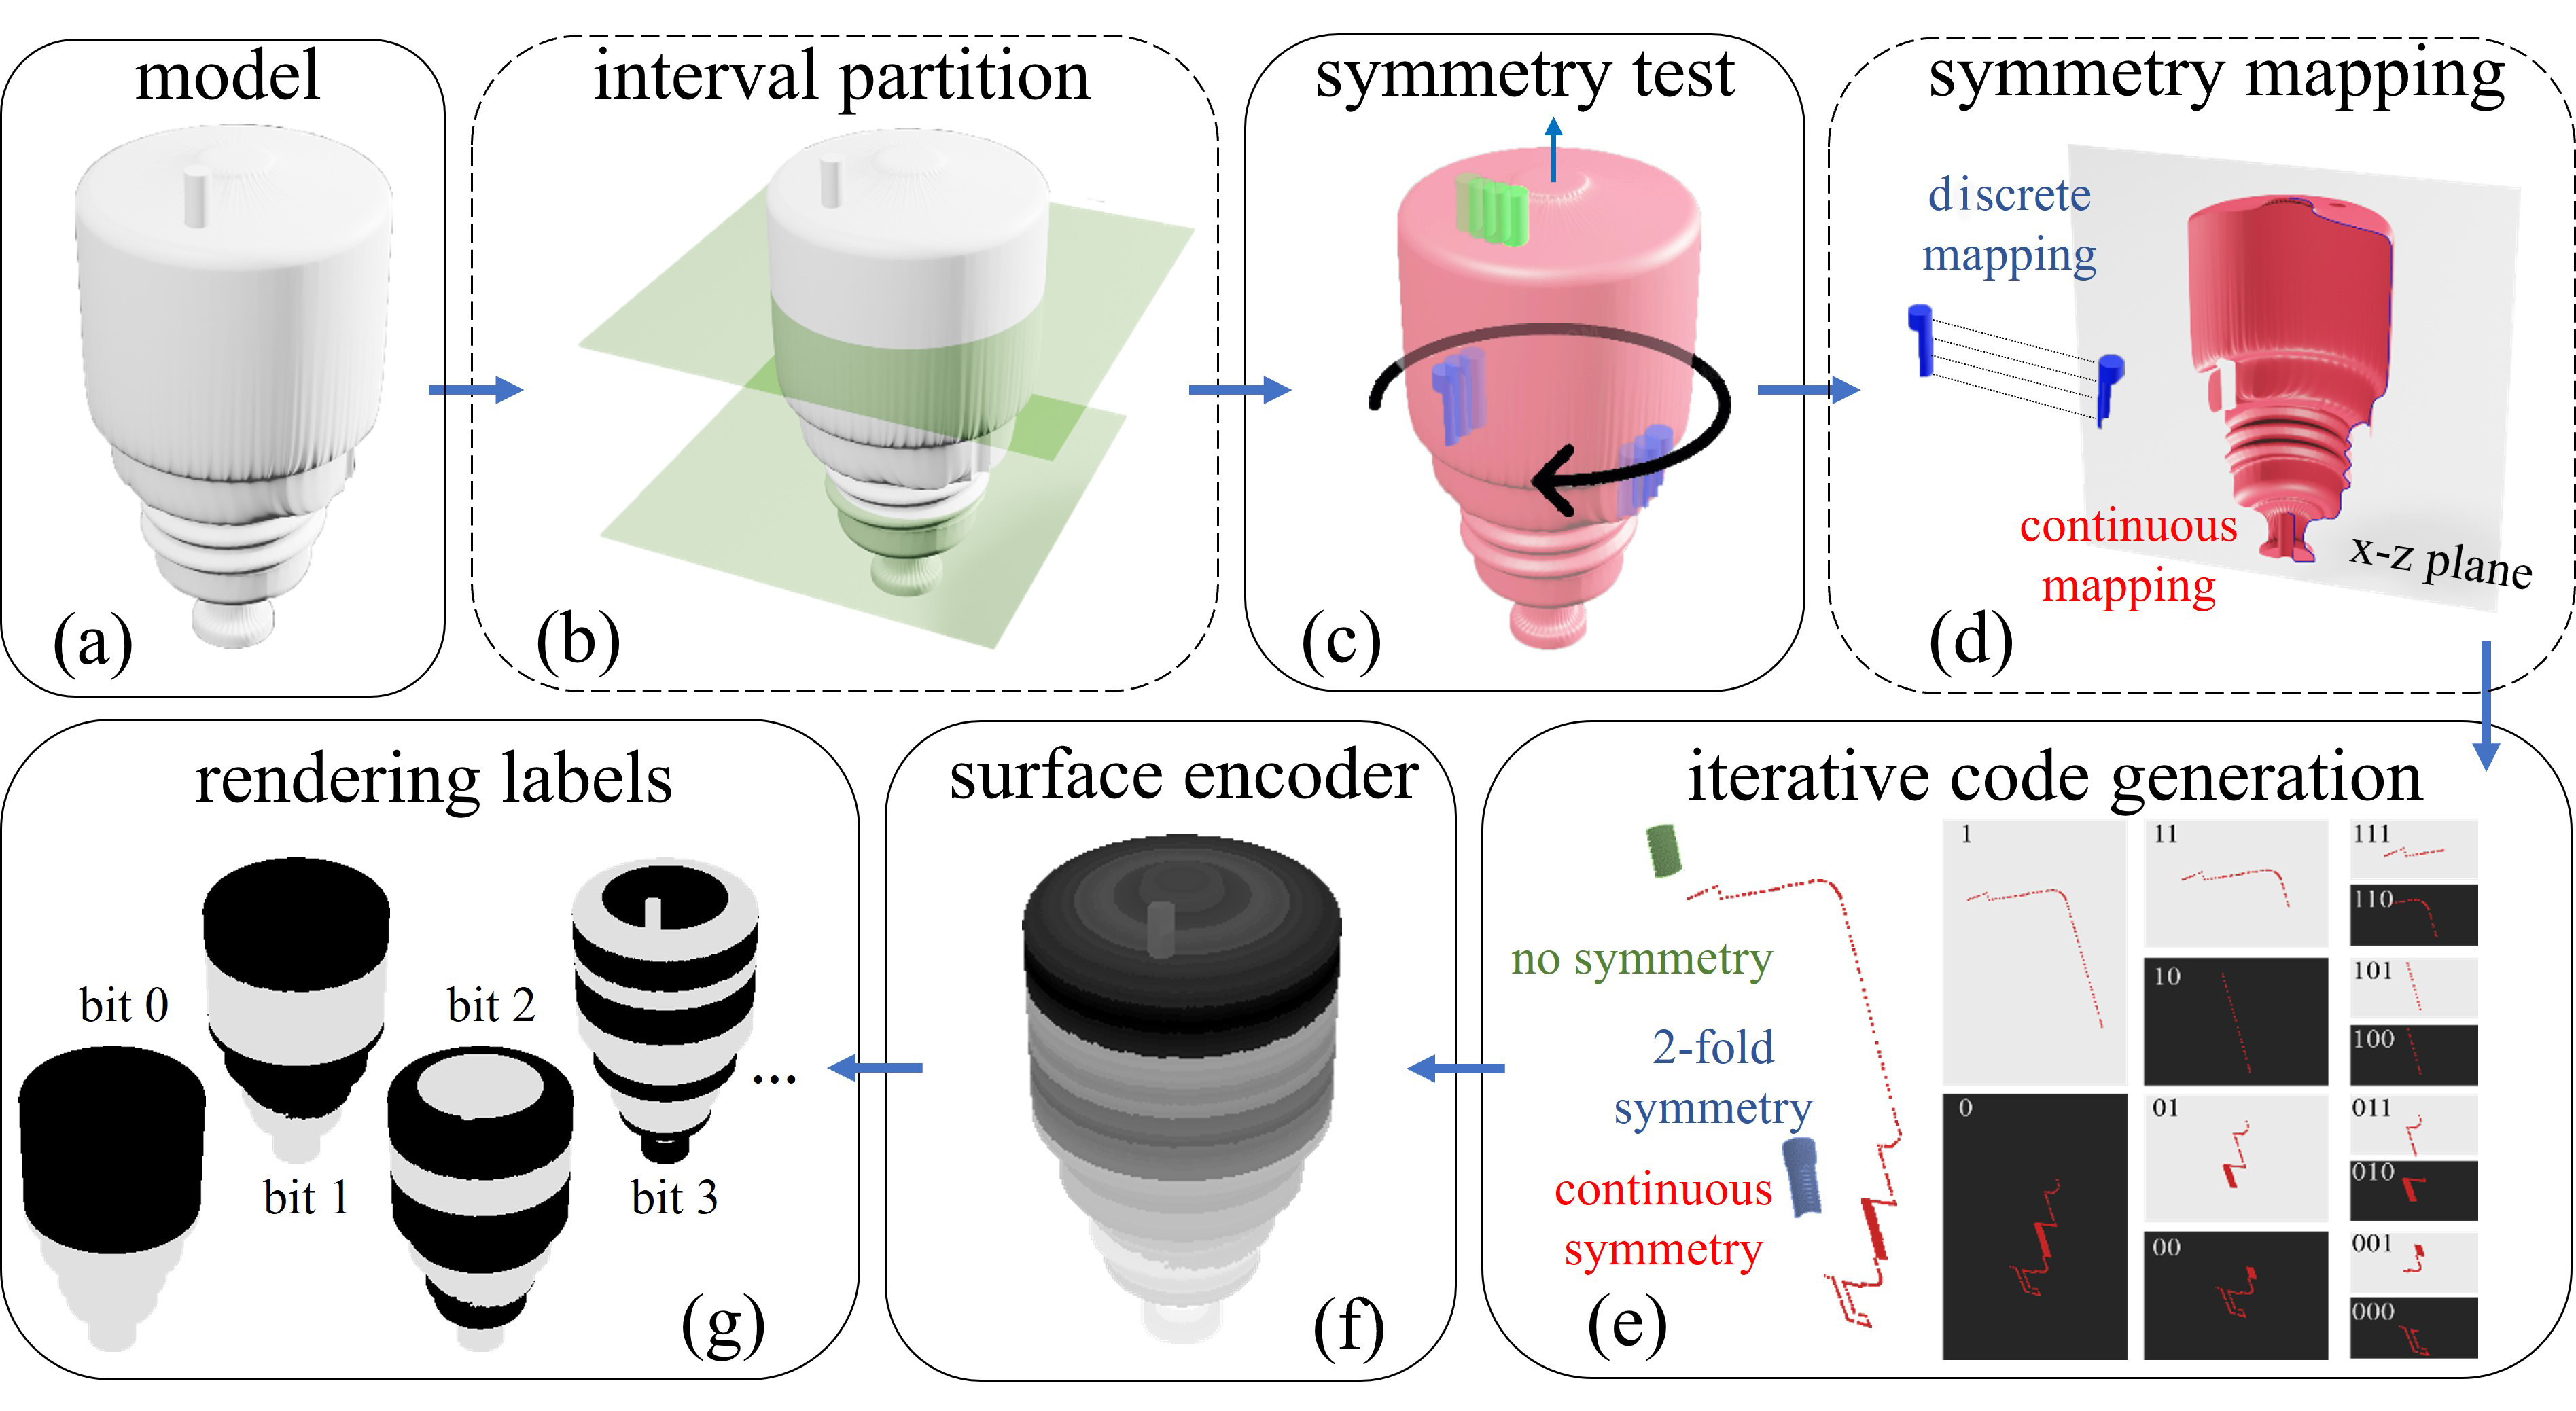
\includegraphics[width=0.83\textwidth]{figure/symnet/process_of_model.jpg}}
        \caption{\textbf{SymCode生成过程和标签渲染。} (a) 物体CAD模型。 (b) 对于复杂模型,我们手动将模型划分为几个部分,以确保后续过程的更高精度。 (c) 基于对称优先级测试顶点的对称类型。 (d) 找到每个一对多对应关系的主顶点;连续对称性和离散对称性分别处理。 (e) 每个对应关系分配一个唯一的二进制代码 $\mathbf{c}_i$。 (f) 表面编码器使用二进制代码对模型中的每个顶点进行编码,固有地保留对称信息。 (g) 渲染的标签用作网络的中间目标。 可选过程用虚线框表示。}
        \label{process_of_model}
\end{figure}

\subsection{考虑对称的表面编码}
我们的目标是使用离散二进制代码 $\mathbf{c}_r$ 对每个一对多对应关系 $\mathbf{o}_r$ 进行编码。~\Cref{process_of_model} 展示了所提出的一对多表面编码流程的示意图。

\textbf{生成一对多对应关系 } 当一个物体具有对称性时,存在多个刚体运动可以将一个真实姿态映射到其他真实姿态。形式上,我们将集合表示如下:
\begin{equation}
\mathcal{M} = \{\mathbf{m}\in SE(3)\ |\ \mathbf{T}_1 \cdot \mathbf{m} \in \{\mathbf{T}_1, \mathbf{T}_2,..., \mathbf{T}_n\} \}
\label{eq:rigid_motions}
\end{equation}
其中 $\mathbf{T}_1$ 表示任意一个真实姿态,$\mathbf{T}_k$ 表示另一个真实姿态,$n$ 表示可能的真实姿态的总数。

对称性可以分为两类:离散对称和连续对称。对于离散对称,集合 $\mathcal{M}$ 包含有限数量的元素。对于顶点 $\mathbf{P}$,我们生成属于同一一对多对应关系的所有其他可能的3D顶点,如下所示:

\begin{equation}
\mathbf{P}_{j,k}=\mathbf{m} \cdot \mathbf{P},\quad k=1,2,..,n, \quad \mathbf{m} \in \mathcal{M}\label{eq:generate_correspondence}
\end{equation}

% 注意,提供的模型表面上不一定存在 $\mathbf{P}_{j,k}$。为了确保模型中的每个顶点都有对应的对方,如果它们尚不存在,我们将把相应的顶点 $\mathbf{P}_{j,k}$ 添加到模型表面。此步骤确保模型中的每个顶点在一对多对应关系中都有其对应的对方。随后,属于一对多对应关系的顶点将根据 \Cref{eq:generate_correspondence} 进行分组。

对于连续对称性,表面的顶点沿对称轴旋转,最终在一个平面上对齐,如~\Cref{process_of_model}(d)所示。通过这样做,旋转后在平面上同一位置的顶点被合并到同一个对应关系中。我们可以将旋转过程形式化如下:

\begin{equation}
\tilde{\mathbf{P}}=
\begin{bmatrix}
 \sqrt{x^2+y^2}  &0 &z
\end{bmatrix}^T
\label{eq:rotation_projection}
\end{equation}

这里,$\tilde{\mathbf{P}}$ 是原始顶点 $\mathbf{P}$ 的转换顶点,被称为主顶点。$x, y, z$ 分别表示 $\mathbf{P}$ 的三个分量。假设旋转发生在 z 轴上,结果平面是 x-y 平面,如~\Cref{process_of_model}(d) 所示。

\textbf{处理多种对称形式 } 对于T-LESS数据集,不同的物体仅标注了主要的对称类型。我们可以直接基于这种对称性注释生成一对多对应关系。然而,许多物体由对称部分的混合体组成。考虑一个由立方体和圆柱体组合而成的物体。虽然考虑整个物体可能表明离散对称性,但在遮挡场景中使用基于离散对称性构建的对应关系仍会导致歧义。

此外,一些物体被认为是“几乎对称的”,即它们除了一个小细节外表现出对称性。为了解决这些挑战,我们提供了一个高级注释工具,使物体模型的标注更加精确。这是整个过程中唯一仍需手动完成的部分,但只需几分钟即可完成。如果物体是完全对称的,则不需要此步骤,从而使整个注释过程完全自动化,依赖于BOP~\cite{hodan2024bop}的对称性注释信息。

\Cref{process_of_model}(a) 提供了这种情况的示例。我们明确地将物体上的点分类为以下四类:(1) 无对称性,(2) 连续对称性,(3) 离散对称性,和 (4) n 重对称性。n 重对称性是离散对称性的一个特例,即对称角度为
\begin{equation}
\theta=i \cdot 2\pi /n,\quad i \in \{1,...,n\}
\end{equation}
沿轴线。分类是通过每个顶点与应用 \Cref{eq:generate_correspondence} 变换后的最近顶点之间的平均距离来确定的。由于不同类型的对称性本质上具有包含关系,连续对称性包含在离散对称性中,离散对称性包含在 n 重对称性中,而不属于上述任何类型的顶点将被视为无对称性。我们按以下顺序评估对称性:连续对称性、离散对称性、n 重对称性,最后是无对称性,我们称之为对称优先级。主要对称类型在数据集的元信息中提供。然而,对于破坏对称性的细节,需要人工干预来指定它们并确保识别出正确的对称类型。此外,还可以使用从经验或实验观察中得出的误差阈值来辅助识别对称类型 $sym$。对于给定的对称类型 $sym$,我们将基于该对称性生成对应关系集 $\mathcal{M}$ 并计算在此特定对称类型 $sym$ 下的误差如下:

\begin{equation}
\mathbf{e}_{j,sym} = \sum_{m\in\mathcal{M}}\left \|  \mathbf{P}_{\text{near}} - \mathbf{m}\mathbf{P} \right \| 
\end{equation}
其中 $\mathbf{P}_{\text{near}}$ 是指物体表面上与变换顶点 $\mathbf{m}\mathbf{P}$ 最近的顶点。

在移除属于高优先级对称性的顶点后,剩余的顶点可以分类到低优先级对称性类别中。任何未分类为任何对称性类型的顶点将被识别为无对称性。

为了获得更精确的分类,可以将模型细分为更小的区间,从而在每个区间内识别不同形式的潜在对称性。这种方法允许对对称结构进行更详细的分析,如\Cref{process_of_model}(b)所示。

\textbf{对应关系编码 } 我们已经建立了一对多对应关系集 $\mathbf{O}_\text{sym}$,其中每个组 $\mathbf{Y}_j$ 包含顶点 $\mathbf{P}_{j,k}$。此外,每个组 $\mathbf{Y}_j$ 都与一个对称类型 $sym$ 相关联。我们引入了一种对一对多对应关系集进行编码的方法。物体表面通过为一对多对应关系集引入分层二进制分组方案进行编码。

编码表示该像素匹配到的对应组 $\mathbf{Y}_j$。编码应理想地满足以下标准:1)为了提供足够的信息进行姿态估计,对于具有不同对称类型的两个组 $\mathbf{Y}_j$ 和 $\mathbf{Y}_j'$,编码应表现出显著差异。2)为了便于网络学习,彼此接近的对应关系应具有更相似的编码。3)每个 $\mathbf{Y}_j$ 对应一个唯一的编码。
通常,我们从每个对应关系中选择一个3D顶点,称为主顶点,同时考虑邻近对应关系的空间接近性。主顶点将在下一步中用于实现二进制编码。

接下来,我们介绍如何为每个对应关系获取主顶点。对于具有连续对称性的对应关系,我们使用~\Cref{eq:rotation_projection} 将顶点映射到平面上,选择该顶点作为主顶点。对于其他类型的对称性,我们基于以下简单标准选择主顶点,该标准可以替换为其他满足条件(2)的方法。在我们的实现中,所使用的标准计算每个对应关系中每个顶点的各坐标分量的绝对值之和。然后根据以下公式选择主顶点,记为 $\tilde{\mathbf{P}}$:
\begin{equation}
    \tilde{\mathbf{P}} = \max_{\mathbf{P}_{j,k}}
    (\left | x_{j,k} \right | +\left | y_{j,k} \right | +\left | z_{j,k} \right |), \quad \mathbf{P}_{j,k} \in \mathbf{Y}_j
\end{equation}

如~\Cref{process_of_model}(e)所示,该物体的主顶点由彩色顶点表示。在对应关系中,只有一个顶点不是对称的,它将作为主顶点,颜色为绿色。
对于连续对称性,主顶点(红色)位于通过~\Cref{eq:rotation_projection}计算的平面上。
对于2重对称性,坐标值较高部分的顶点将作为主顶点,颜色为蓝色。

\textbf{迭代编码生成 } 这一部分的灵感来自于一对一对应方法中使用的二进制编码~\cite{su2022zebrapose}。给定一对多对应关系集,我们希望用一个二进制代码 $\mathbf{c}_i \in {0, 1}^d$ 来表示每个对应关系 $\mathbf{o}_i$,其中 $d$ 是二进制代码的长度。我们基于每个对应关系的主顶点构建这样的编码。

在\Cref{process_of_model}(e)中,我们展示了执行 $d$ 次主顶点分组迭代的过程。分组迭代从所有主顶点的集合 $G$ 开始。对于具有二进制代码 $\mathbf{c}_i$ 的组 $G_{i}$,我们使用 k-means 将其分成两组。结果组被分配代码 $\mathbf{c}_i \ll 1$ 和 $(\mathbf{c}_i \ll 1) + 1$,其中操作 $\ll$ 表示二进制左移。最终,我们获得 $2^d$ 个组,每个组都有其二进制代码。这些二进制代码可以用从 $0$ 到 $2^d - 1$ 的十进制形式表示。表面编码器如\Cref{process_of_model}(f)所示,其中颜色表示二进制代码 $\mathbf{c}_i$ 的十进制值。

\subsection{网络架构}
\begin{figure}[t]
    \centerline{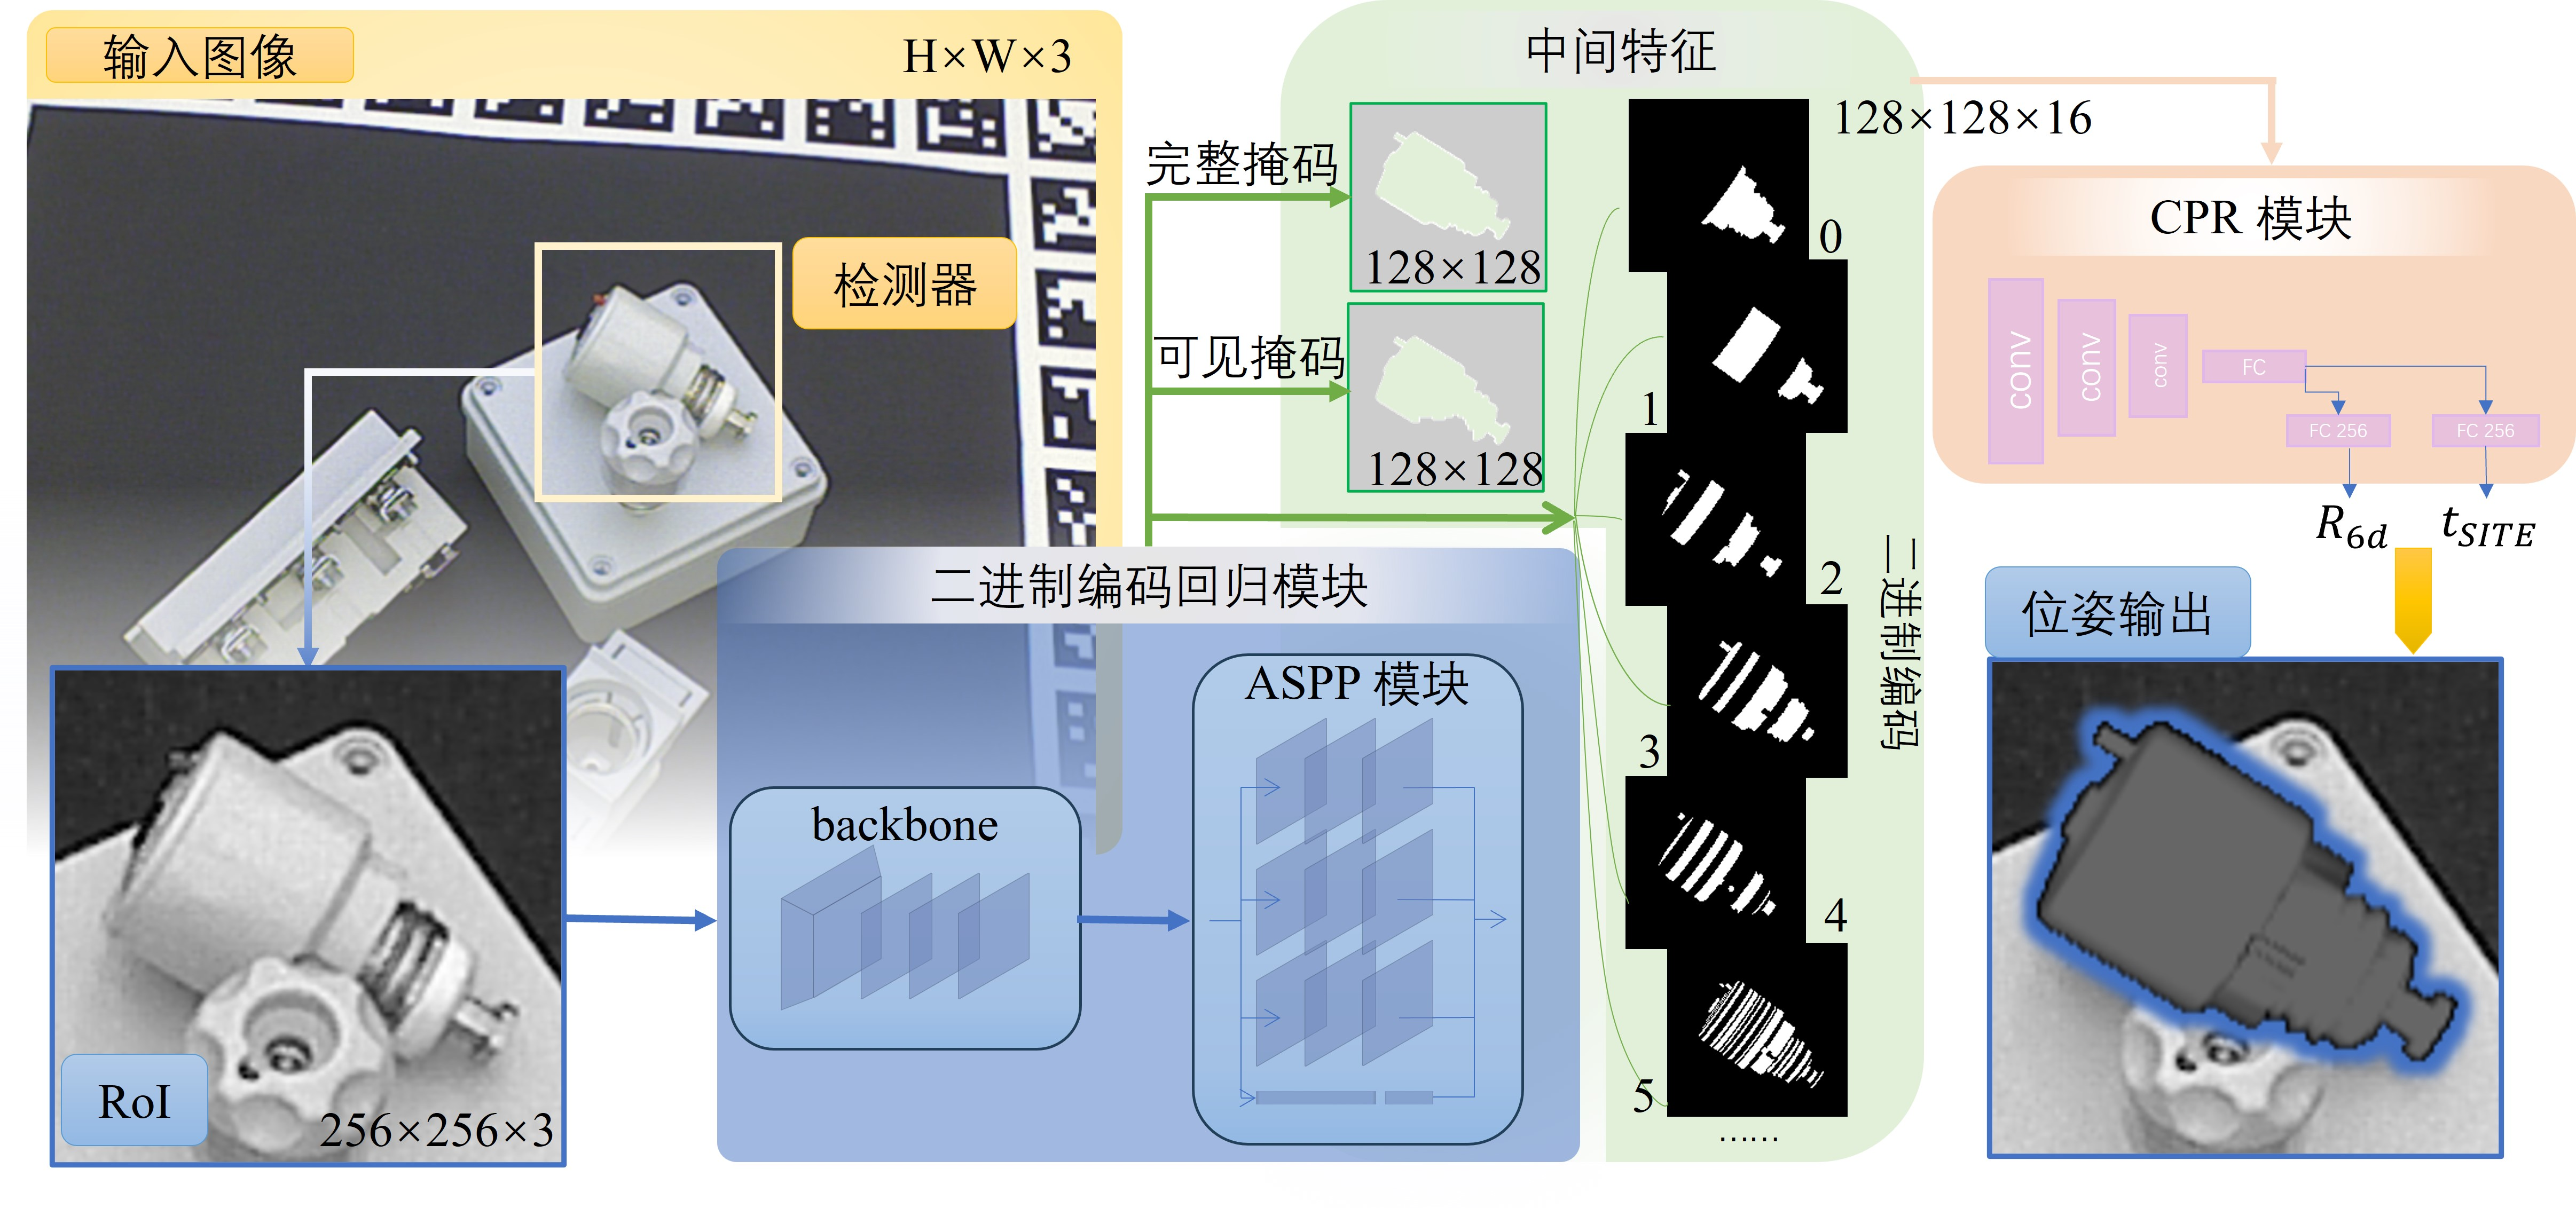
\includegraphics[width=1.0\textwidth]{figure/symnet/network.jpg}}
    \caption{SymNet框架 给定一张RGB图像,我们的SymNet以放大的兴趣区域(RoI)作为输入,并预测包括掩码和二进制编码图在内的中间特征。然后,CPR模块直接回归6D物体姿态。整个过程是一个端到端的过程,消除了对PnP的精细化或RANSAC过程的需求。}
    \label{fig:network}
\end{figure}

我们的网络灵感来自于ZebraPose~\cite{su2022zebrapose}和GDR-Net~\cite{wang2021gdr}。在\Cref{fig:network}中,我们为二进制编码模块提供了一个尺寸为$256 \times 256 \times 3$的放大兴趣区域(RoI)。输出的中间变量包括尺寸为$128 \times 128$的无模态掩码$M_{\text{amo}}$、尺寸为$128 \times 128$的可见掩码$M_\text{{vis}}$和尺寸为$128 \times 128 \times 16$的SymCode图。随后,这些中间变量被用作对应关系姿态回归(CPR)模块的输入。

二进制编码模块包括一个ResNet-34骨干网络~\cite{he2016resnet},并利用了空洞空间金字塔池化(ASPP)\cite{chen2017deeplabv3},该方法在并行的空洞卷积中对特征进行不同尺度的重采样非常有效。我们还尝试了不同的卷积策略和来自CDPN\cite{li2019cdpn}的上采样方法作为网络架构的一部分,但结果没有显著差异。

我们利用一个简单的基于对应关系的姿态回归(CPR)模块,直接从可见掩码 $M_\text{{vis}}$、无模态掩码 $M_{\text{amo}}$ 和 SymCode 图 $M_\text{code}$ 回归6D姿态。CPR模块包括三个卷积层,每个卷积层后面跟着组归一化和ReLU激活。随后,两个全连接层应用于展平的特征。最后,两个并行的全连接层分别输出参数化为 $\mathbf{R}_{6d}$~\cite{zhou2019continuity} 的3D旋转和参数化为 $\mathbf{t}_\text{SITE}$~\cite{li2019cdpn} 的3D平移。总体而言,我们网络的总参数量为 $63.2M$。

我们对可见掩码、无模态掩码和SymCode图使用$L1$损失。我们的训练损失定义为
\begin{equation}
    Loss = L_\text{masks} + L_\text{code} + L_\text{params} + L_\text{ADD-S}
\end{equation}
$L_\text{params}$ 对应于端到端训练的损失,使用$L1$损失来处理 $\mathbf{R}_{6d}$ 和 $\mathbf{t}_\text{SITE}$。此外,$L_\text{ADD-S}$ 项源自PoseCNN的工作~\cite{xiang2018posecnn}。

在训练过程中,所有损失同时进行训练,没有任何参数被冻结。在我们的初步实验中,我们还探索了一种非端到端的训练策略,其中 $L_\text{masks} + L_\text{code}$ 用于训练二进制编码模块,而 $L_\text{params} + L_\text{ADD-S}$ 仅用于训练 CPR 模块;然而,这导致了结果的轻微下降。

